%----------------------------------------------------------------------------------------
%	SLIDE 7.
%----------------------------------------------------------------------------------------
\begin{frame}
\frametitle{Solutions for all $r$ values}
\framesubtitle{Final form og $\omega (r)$}

\begin{itemize}
	\item From this, dimensional analysis can show the true relationship between frame-dragging and rotation of the star:
	\begin{block}{}
		\begin{equation} \label{eq:9}
			\omega (r)
			=
			\frac{2 J}{r^{3}}
			=
			\frac{2 I \Omega}{r^{3}}, \quad r \geq R
		\end{equation}
	\end{block}
	\item From \eqref{eq:8} and \eqref{eq:9}, $\omega (r)$ can be finally described for every $r$ values.
\end{itemize}
\begin{figure}
	\centering
	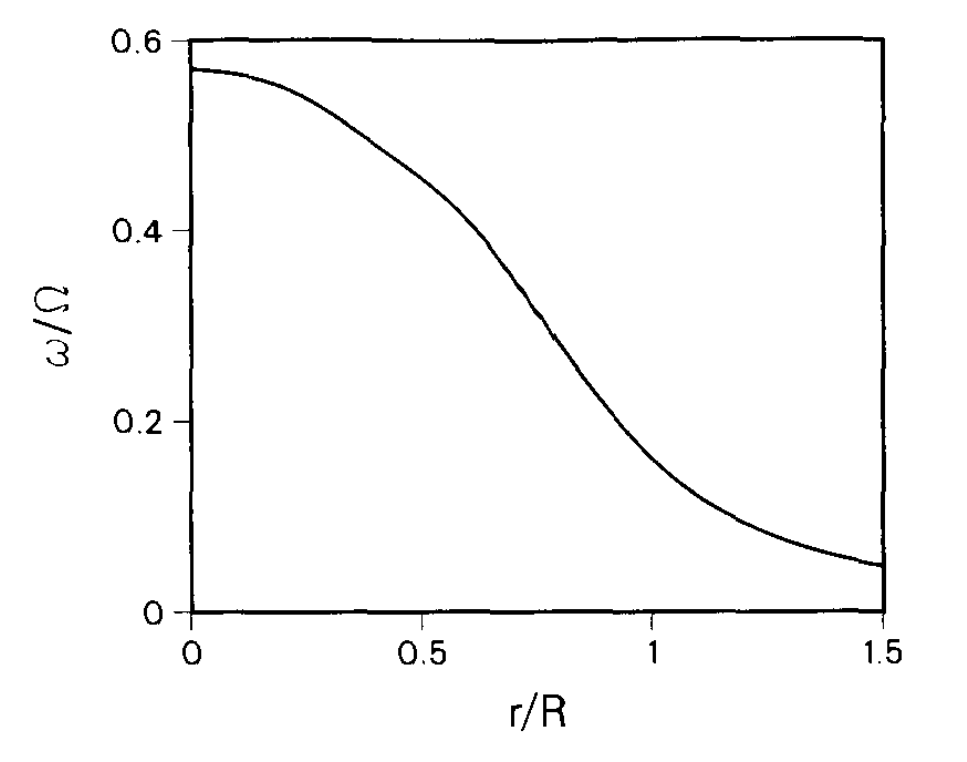
\includegraphics[width=0.45\linewidth]{./images/ns-omega.png}
\end{figure}

\end{frame}
